\documentclass{beamer}
\usetheme{Frankfurt}
\usepackage[utf8]{inputenc}

\usepackage{algorithmic}
\usepackage{algorithm}
{\renewcommand{\bibname}{References}}  
\usepackage[backend=bibtex,style=numeric]{biblatex}  %backend=biber is 'better
\renewcommand{\algorithmicrequire}{\textbf{Input:}}
\renewcommand{\algorithmicensure}{\textbf{Output:}}

\usepackage{amssymb}
\usepackage{amsfonts}
\usepackage{amsmath}
\newcommand{\argmin}{\mathop{\mathrm{arg\,min}}\limits}
\newcommand{\argmax}{\mathop{\mathrm{arg\,max}}\limits}
\newcommand{\mymin}{\mathop{\mathrm{min}}\limits}
\addbibresource{references.bib}  

\graphicspath{ {./images/} }

\usepackage{xspace}

\usepackage{multirow}
\usepackage{booktabs}

\title[A GRASP metaheuristic for a TDP]
{A GRASP metaheuristic for a territorial design problem in financial institutions}
\author{Eduardo Salazar, Roger Z. Ríos}
\institute[]{
    Department of Mechanical and Electrical Engineering \\
    Universidad Autónoma de Nuevo León \\
    San Nicolás de los Garza, N.L.
}
\date[X CSMIO]{
    X Congreso de la Sociedad Mexicana de Investigación de Operaciones \\ 
    October 20th, 2022
}
\begin{document}

\begin{frame}
    \titlepage
\end{frame}

\begin{frame}{Outline}
    \tableofcontents
\end{frame}

\section{Problem statement and motivation}

\begin{frame}{Territorial Design Problem}
    \framesubtitle{Problem formulation}
    According to literature \cite{cor2009}, the main goal of a classic Territorial Design Problem is to minimize the sum of the distances of the $B$ Basic Units (BUs henceforth), which represent clients, to their $P$ territory centers that are selected out of $S$ possible  centers, fulfilling the specific demands of the BUs whilst taking into consideration several constraints that represent things such as unique assignments, metrics of BUs and their centers.
\end{frame}

\begin{frame}{Financial institution's special requirements}
    \framesubtitle{Problem formulation}
    Following the only available example in previous literature \cite{jimo2020}, financial institutions have specific needs which translate to unique constraints. \\
    For example, each territory center has a specific $S_k$ type of facility (gas station = $S_1$, supermarket = $S_2$, etc), with the number of centers with type $k$ to be contained within lower and upper bounds $L_k$ and $U_k$, respectively, for $k \in 1\ldots5$ \\
    Another value to be balanced between the territories is a risk parameter $R$ associated with each BU, with each territory having a given $\beta$ threshold of risk which cannot be exceeded.
\end{frame}

\begin{frame}{Financial institution territory example}
    \framesubtitle{Instance example}
    $B = 15$ \\
    $S = 8$ \\
    $P = 4$ \\
    \begin{figure}
        \centering
        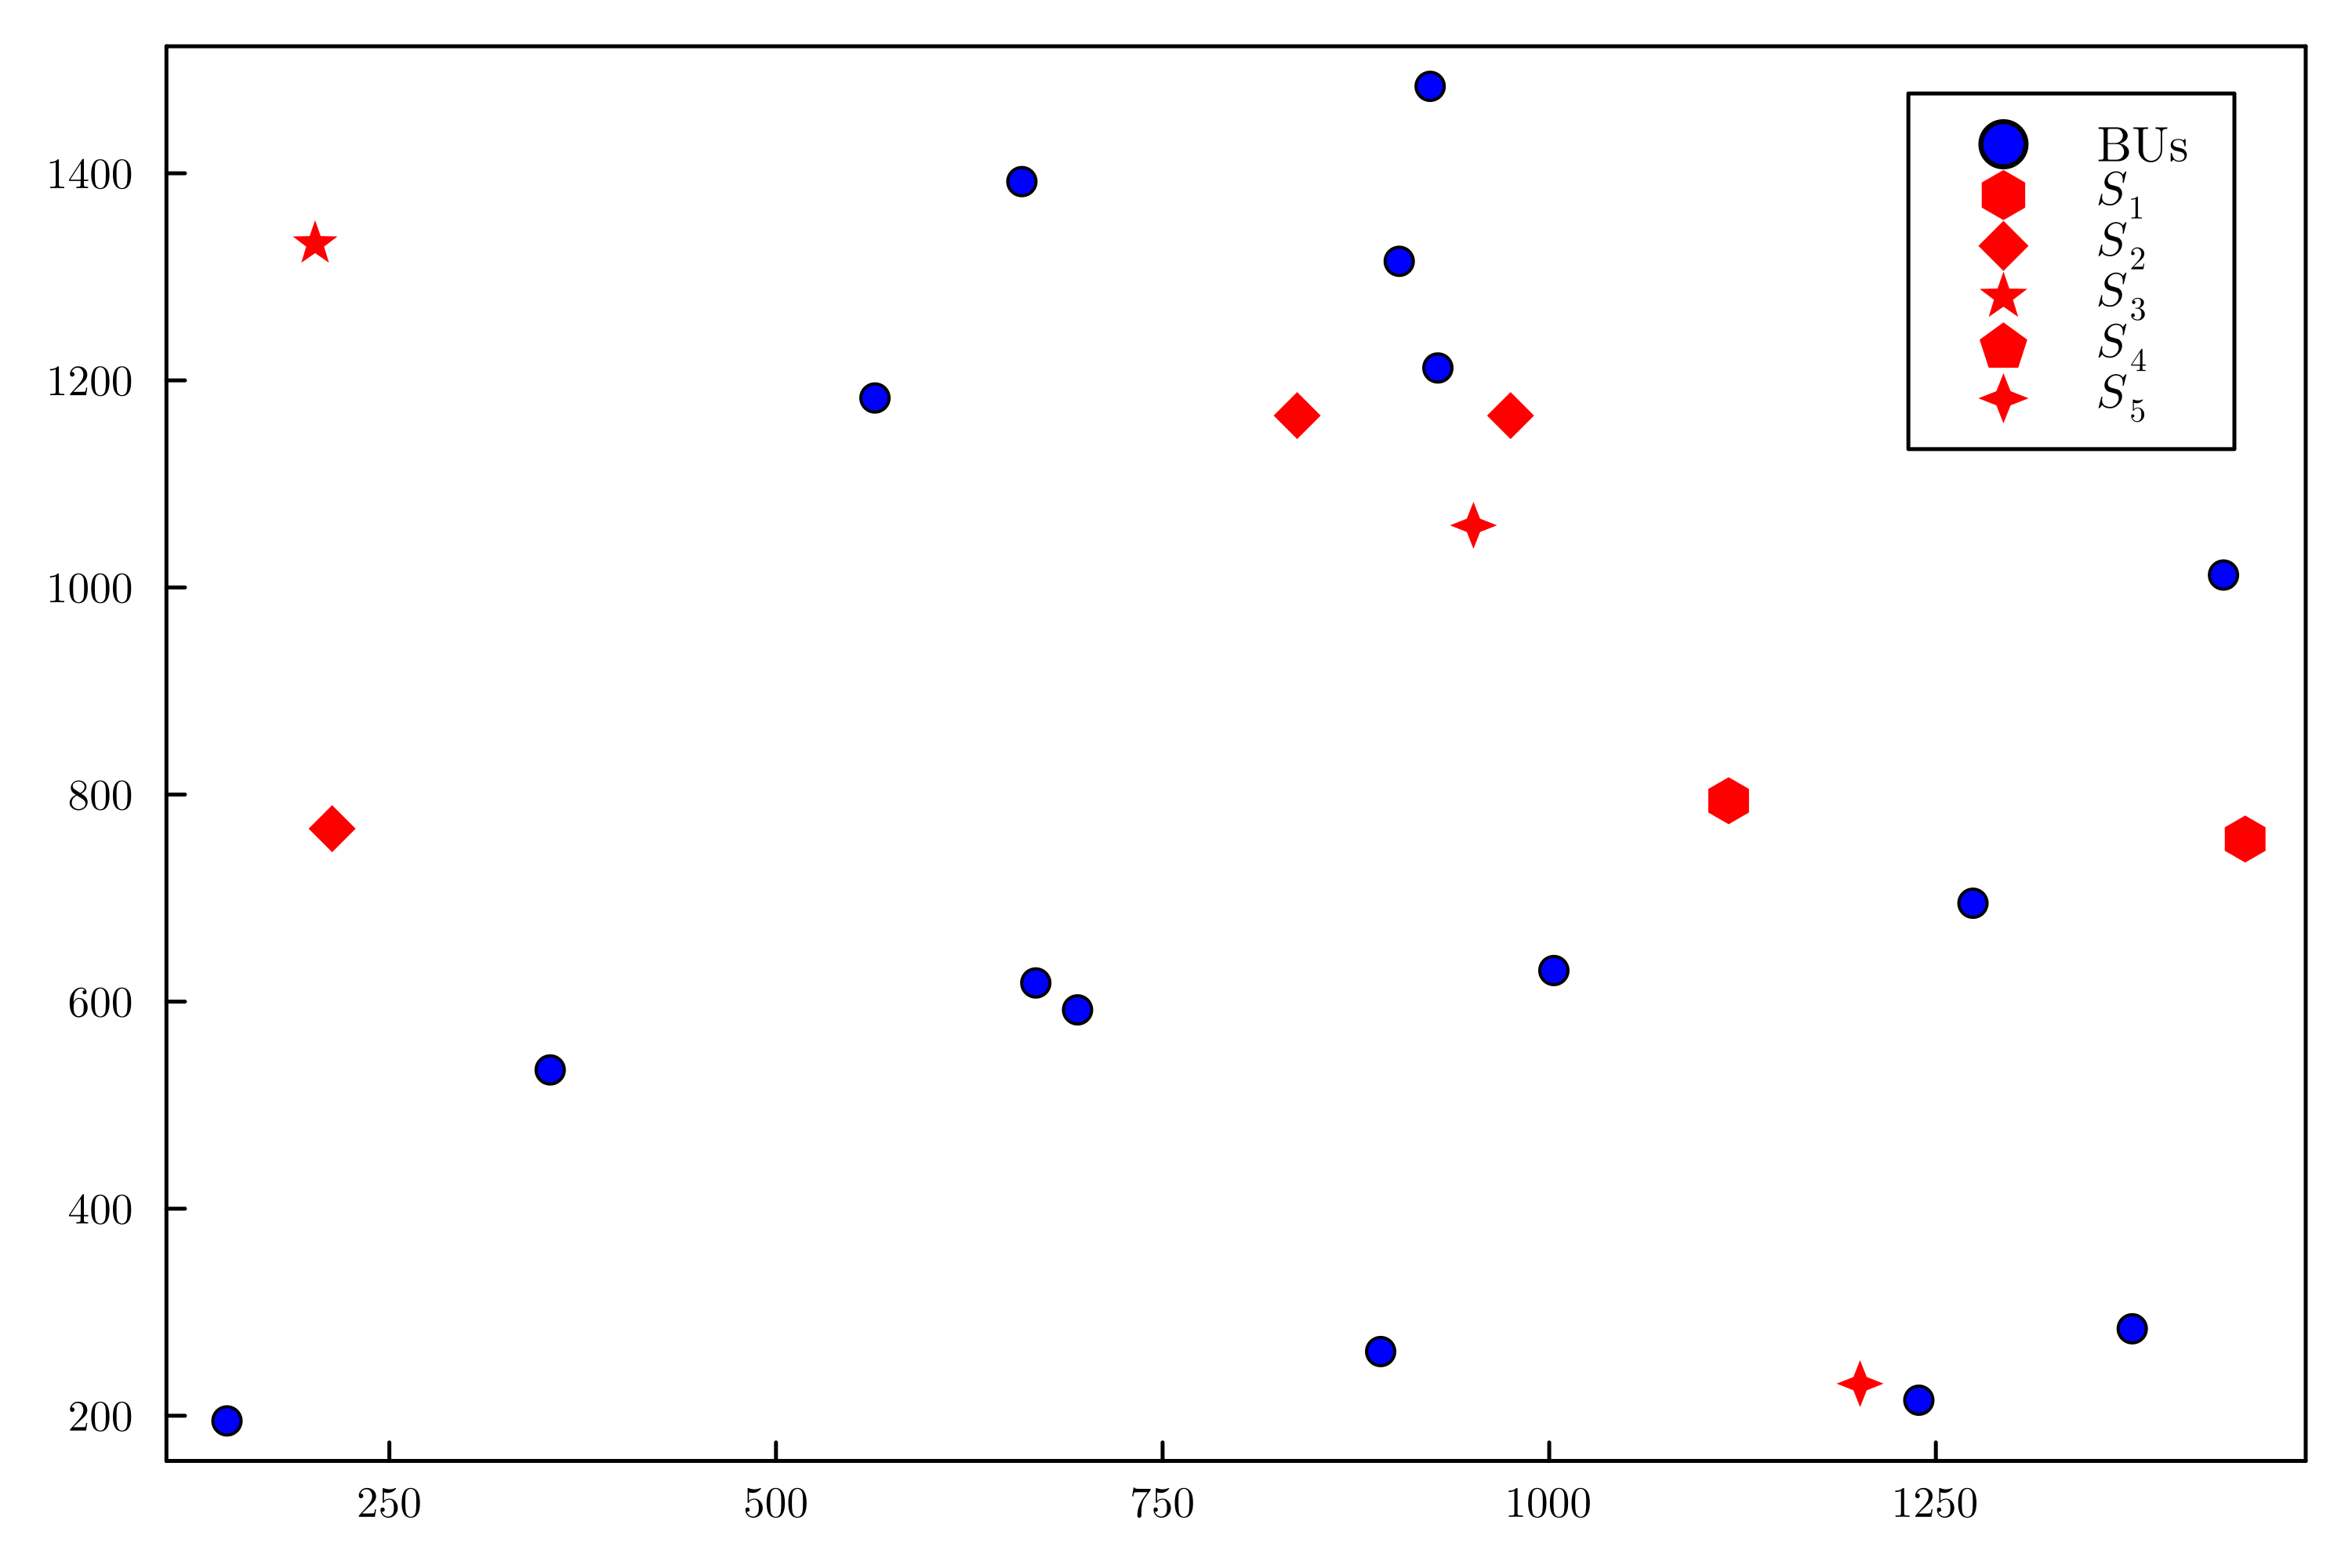
\includegraphics[scale=0.082]{plot_instance.png}
        \label{fig:instancia}
    \end{figure}
\end{frame}

\begin{frame}{Financial institution territory example}
    \framesubtitle{Solution example}
    $B = 15$ \\
    $S = 8$ \\
    $P = 4$ \\
    \begin{figure}
        \centering
        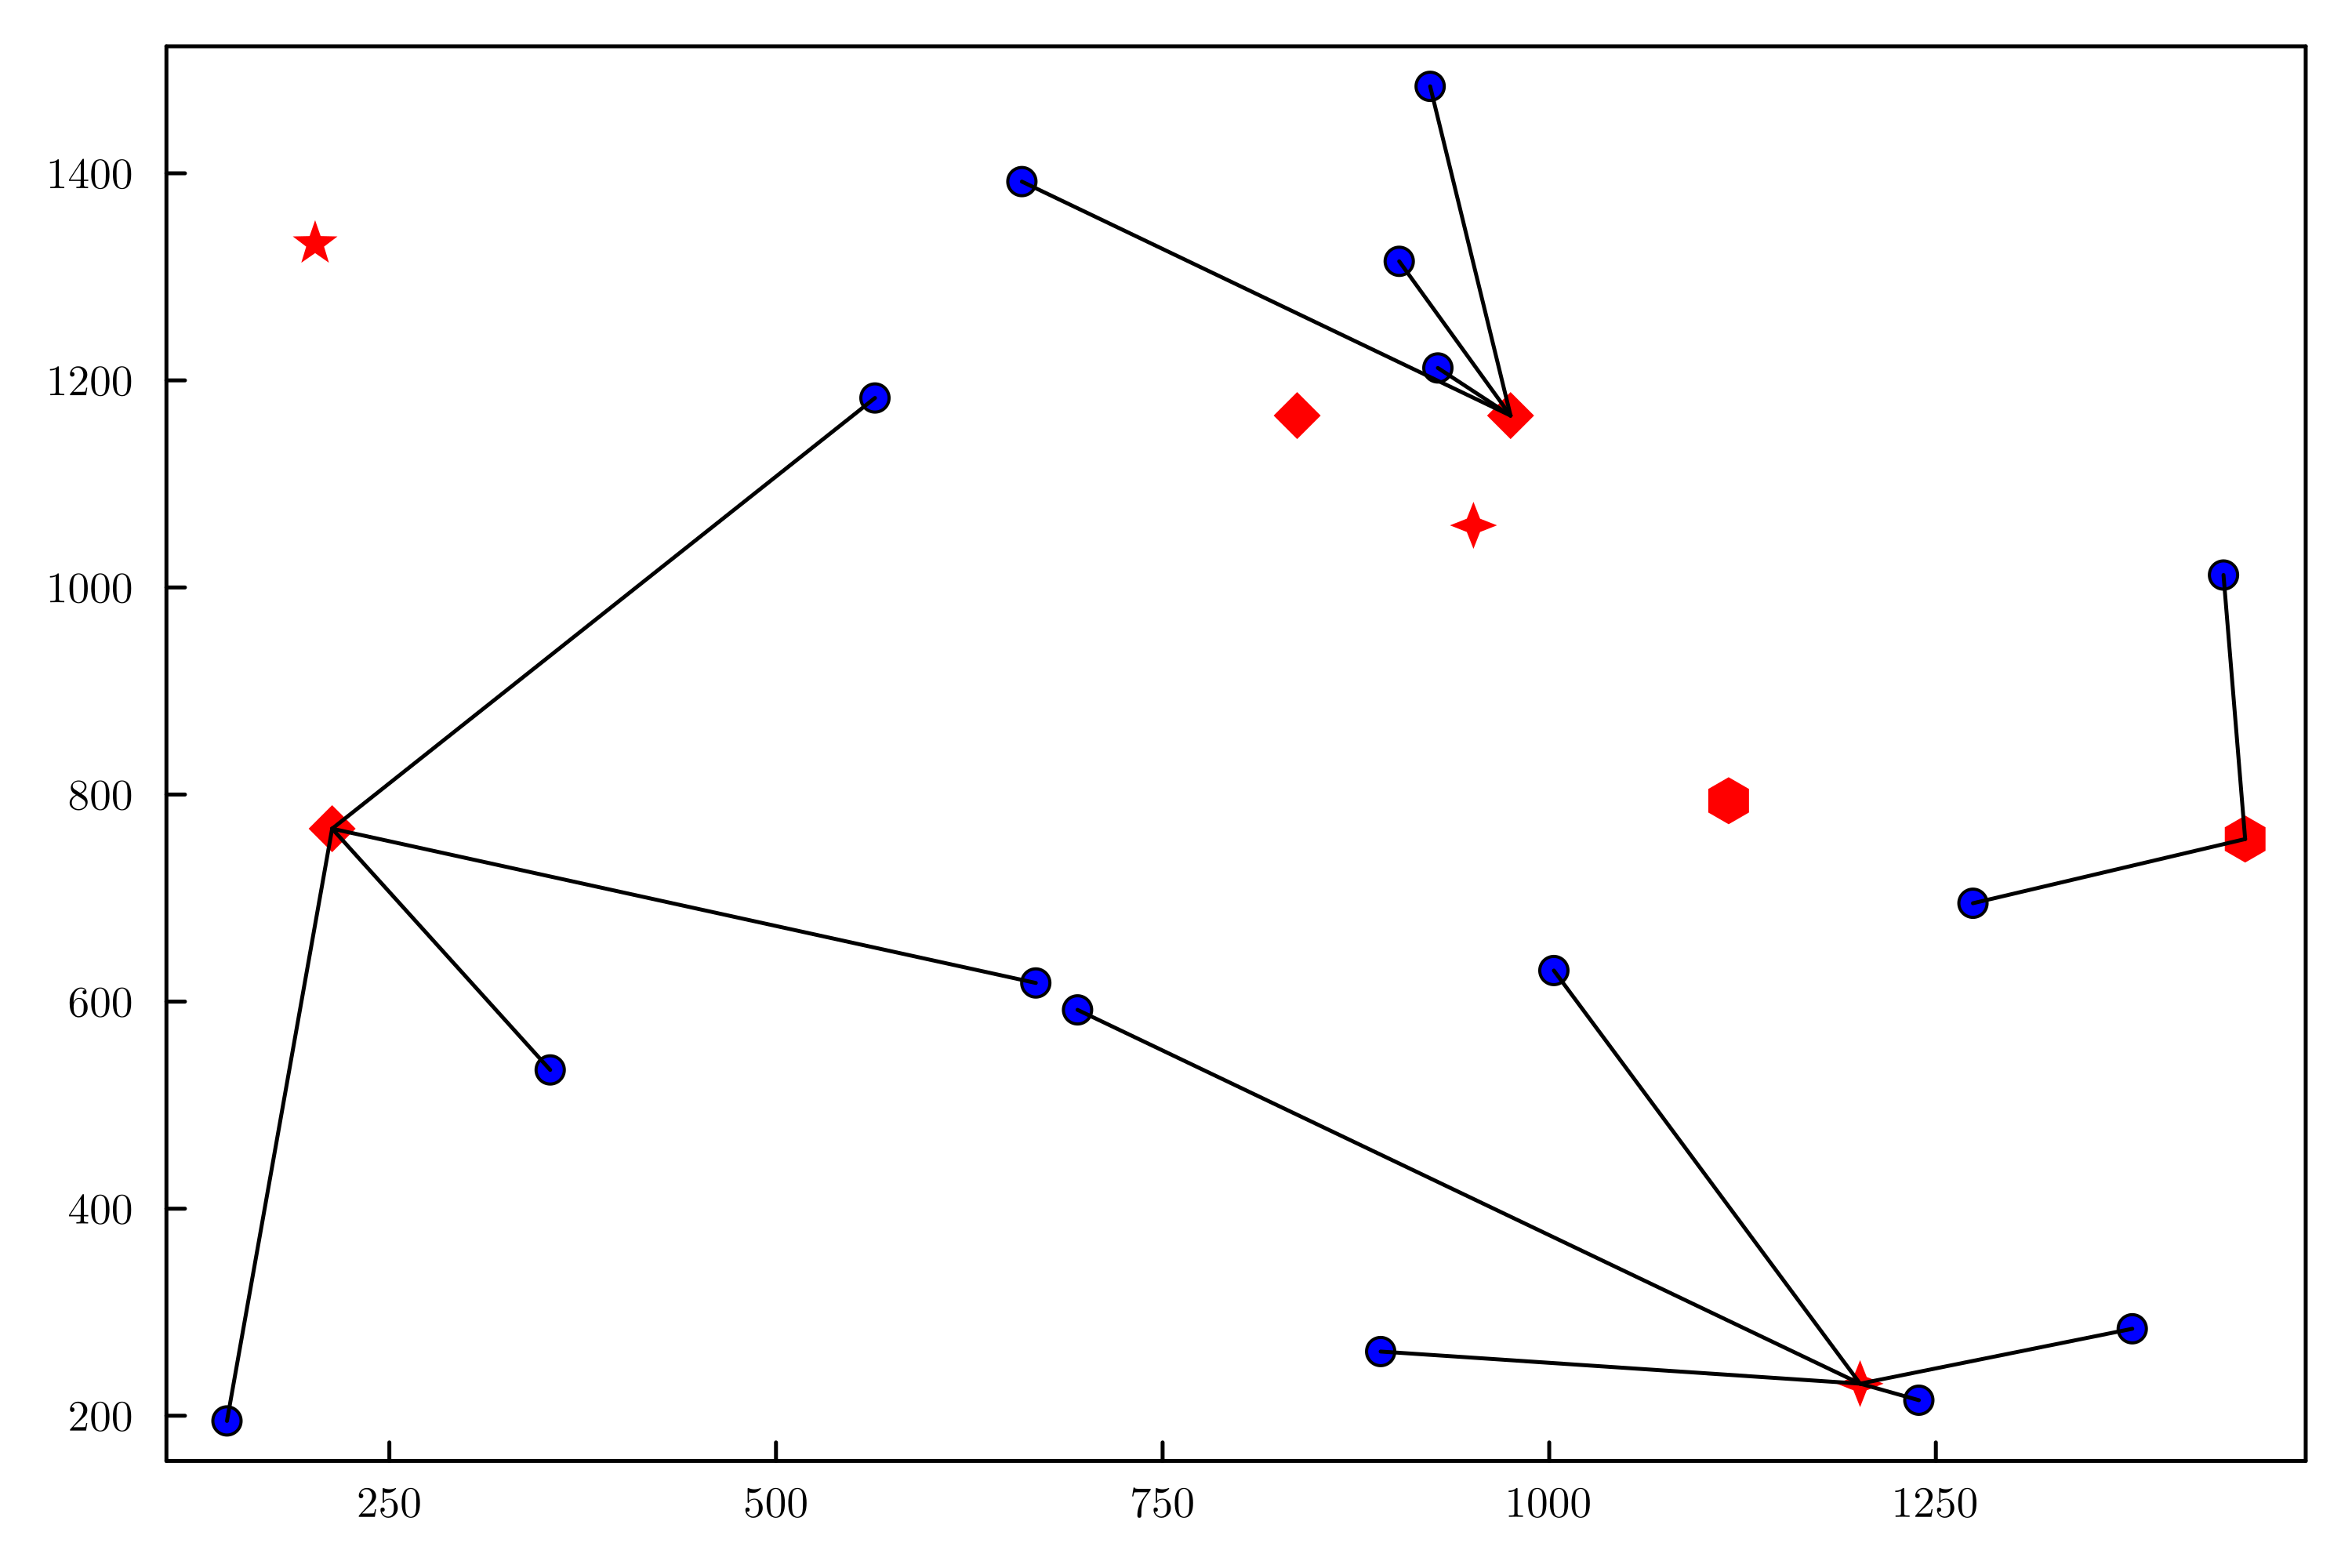
\includegraphics[scale=0.082]{solution_example.png}
        \label{fig:solucion}
    \end{figure}
\end{frame}


\begin{frame}{Applications}
    \begin{figure}
        \centering
    \end{figure}
   As stated before, the purpose of this model is to provide a generalization for financial institutions that wish to design the territories representing where to open a facility and which clients will be served by that facility. Risk balancing among the facilities is extremely important for such type of business, as a failure in a single facility node can compromise the entire network.
\end{frame}

\begin{frame}{Motivation and Purpose}
    The model described in this work is motivated by a previous model described in \cite{jimo2020}. However, there are several differences between both. In this model, the risk balancing is modelled as a constraint whereas the other model presents it as part of the objective function. Moreover, the other model was applied to an existing territorial design so the objective function also contained a term related to keeping as much as possible of the original design. Our model does not take into account the adjacency of BUs as neither a constraint or parameter. \\
    This model can be viewed as a vertex p-center problem with multiple capacity constraints, given that even the uncapacitated vertex p-center problem is NP-hard \cite{eswa2016}, our TDP is also NP-hard \, therefore the perceived usefulness of heuristic approaches for solving it.
\end{frame}

\begin{frame}{Combinatorial model}
    \framesubtitle{Problem formulation}
    \begin{itemize}
        \item Sets and parameters
        \begin{itemize}
            \item $S = \{1, 2, ..., s\}$, set of possible territory centers
            \item $B = \{1, 2, ..., b\}$, set of possible BUs
            \item $D_{ij} = $ distance matrix between center $i$ and BU $j$, $i \in S, j \in B$
            \item $\mu_m^i$ = target of activity $m$ measure at center $i$
            \item $v_m^j$ = measure of activity $m$ at BU $j$
            \item $t_m$ = tolerance of activity $m$ measure
            \item $R_j$ = risk measure at BU $j$
            \item $\beta_i$ = risk threshold at center $i$
            \item $S_k = \{1,2,...,s\}$, 1 if $s$ is of type $k$, 0 if not, $k \in 1\ldots 5$
            \item $L_k, U_k$ = Lower and upper bounds of centers to be used with type $k$
            \item $P$ = Number of centers to be used
        \end{itemize}
        
        \item Variables sets
        \begin{itemize}
            \item \small $Y_i$, binary variable vector where $Y_i$ = 1 if the center $i$ is used, 0 if not.
            \item \small $X_{ij}$, binary variable matrix where $X_{ij}$ = 1 if the BU $j$ is assigned to center $i$.
        \end{itemize}
    \end{itemize}
\end{frame}


\begin{frame}{Mathematical programming}
    \framesubtitle{Formulation}
    Objective Function:
    \begin{equation}
        \mathbf{min}\sum_{i \in S, j \in B}{X_{ij} D_{ij}}
    \end{equation}{}
    Constraints:
    \begin{equation}
       \sum_{i \in S} X_{ij} = 1, \forall j \in B
    \end{equation}{}
    \centering \small Single assignment of a BU $j$ to a center $i$
    \begin{equation}
        X_{ij} \le Y_i, \forall i \in S, j \in B
    \end{equation}{}
    Can only assign BUs to centers that are open
    \begin{equation}
        Y_i\mu_m^i(1-t^m) \le \sum_{j\in B}X_{ij}v_j^m \le Y_i\mu_m^i(1+t^m), \forall i \in S
    \end{equation}{}
    Activity measures for each territory must be within a tolerance range
\end{frame}

\begin{frame}{Mathematical programming}
    \framesubtitle{Formulation}
    \begin{equation}
        l_k \le \sum_{i \in S_k} Y_i \le u_k
    \end{equation}{}
    The selected centers' types must respect the lower and upper bound for each type
    \begin{equation}
        \sum_{i \in S} Y_i = P
    \end{equation}{}
    The number of centers to be opened must be equal to $P$
    \begin{equation}
        \sum_{j \in B}X_{ij}R_j \le \beta_i, \forall i \in S
    \end{equation}{}
    The risk measure of each territory must not surpass the risk threshold
\end{frame}

\section{Proposed heuristic}

\begin{frame}{Proposed heuristic}
    \begin{columns}
        \column{0.65\textwidth}
        \begin{algorithmic}[1]
        
        \REQUIRE $P, \alpha, \gamma, i_{max}$, Instance
        \ENSURE $X,Y$ = binary decision variables
        
        \STATE $A^* \gets \emptyset$
        \STATE $f^* \gets \infty$
        \WHILE {$i_{max} > 0$}
            \STATE $X, Y \gets$ Construct($\alpha, P$, Instance)
            \STATE $X, Y \gets$ LocalSearch($X, Y,$ Instance)
            \STATE $A \gets (X, Y)$
            \IF {$f(A) < f^*$}
                \STATE $f^* \gets f(A)$
                \STATE $A^* \gets A$ 
            \ENDIF
            \STATE $i_{max} \gets i_{max} - 1$
        \ENDWHILE
        \RETURN $A^*$
        
        \end{algorithmic}
        
        \column{0.35\textwidth}
        A metaheuristic framework with a Greedy Randomized Adaptive Search Procedure (GRASP) using a value-based restricted candidate list (RCL).
        Parameters:
        \begin{itemize}
            \item $\alpha$: Threshold quality parameter
            \item $i_{max}$: Number of iterations
            \item $\gamma$: Perturbation parameter.
        \end{itemize}
    \end{columns}
\end{frame}

\begin{frame}{Construction phase}
    The constructive heuristic used in this work consists of two phases: Location and Allocation. \\
    In the Location phase, we must first determine which $P$ centers are to be used out of all the available possible locations. This phase returns the decision variable vector $Y$. \\
    The Allocation phase will allocate which center serves which BU, until all of the clients are allocated to a center. This phase will return the decision variable matrix $X$. \\
\end{frame}

\begin{frame}{Construction phase}
    \framesubtitle{Location heuristics}
    \begin{itemize}
        \item P-dispersion problem
        \item Relaxation of integer constraints
        \item Randomization
    \end{itemize}
\end{frame}

\begin{frame}{Construction phase}
    \framesubtitle{Location heuristics: P-Dispersion Problem}
\scalebox{0.8}{
    \begin{minipage}{1.8\linewidth}
        \begin{algorithmic}[1]
            \REQUIRE $P, S\_coords, S$
            \ENSURE $Y$ := Binary vector of centers to be used
            \STATE $S\_distance \gets $ Euclidean Distance Matrix of all the centers with coordinates $S\_coords$
            \STATE $S\_sol \gets {argmax(S\_distance)}$
            \STATE $T \gets {1...S}$
            \STATE $T \gets T \setminus S\_sol$
            \WHILE {$|S\_sol| < P$}
                \STATE $D \gets []$
                \FOR{$i \in S$}
                    \FOR{$j \in T$}
                        \STATE $D[i] += S\_distance[i,j]$
                    \ENDFOR
                \ENDFOR
                \STATE $max \gets argmax(D)$
                \STATE $S\_sol \gets S\_sol \cup max$
                \STATE $T \gets T \setminus max$
            \ENDWHILE
            \STATE $Y = zeros(S)$
            \STATE $Y \gets Y[idx] = 1, \forall_idx \in T$
            \RETURN Y
        \end{algorithmic}
    \end{minipage}%
    }
\end{frame}
\begin{frame}{Construction phase}
    \framesubtitle{Location heuristics: Relaxation of Integer Constraints}
\scalebox{1}{
    \begin{minipage}{1.8\linewidth}
        \begin{algorithmic}[1]
            \REQUIRE Instance, $P$
            \ENSURE $Y$ := Binary vector of centers to be used
            \STATE $Model \gets$ Build Mathematic Model from Instance
            \STATE $Model.X \gets$ Continous Value {0...1}
            \STATE $Model.Y \gets$ Discrete Value {0,1}
            \STATE $Y \gets Solve(Model)$
            \RETURN Y
        \end{algorithmic}
    \end{minipage}%
    }
\end{frame}

\begin{frame}{Construction phase}
    \framesubtitle{Location heuristics: Randomization}
\scalebox{1}{
    \begin{minipage}{1.8\linewidth}
        \begin{algorithmic}[1]
            \REQUIRE $P$
            \ENSURE $Y$ := Binary vector of centers to be used
            \STATE $Y \gets rand(0:1, P)$
            \RETURN Y
        \end{algorithmic}
    \end{minipage}%
    }
\end{frame}


\begin{frame}{Construction phase}
    \framesubtitle{Allocation heuristics}
    \begin{itemize}
        \item Minimization of distances
        \item Cost of opportunity with restrictions in mind
    \end{itemize}
\end{frame}

\begin{frame}{Minimization of Distances}
    \scalebox{1}{
    \begin{minipage}{1.8\linewidth}
        \begin{algorithmic}[1]
            \REQUIRE $D, Y, B$
            \ENSURE $X$ := binary decision matrix
            \STATE $N \gets [i, \forall_i \in Y == 0]$
            \FOR{$j \in B$}
                \STATE $i \gets argmin(D[:,j]), i \notin N$
                \STATE $X[i,j] \gets 1$
                \STATE continue
            \ENDFOR
            \RETURN $X$
        \end{algorithmic}
    \end{minipage}%
    }
\end{frame}

\begin{frame}{Cost of Opportunity}
    \framesubtitle{Computational results}
    Let us propose a scenario with two centers $i, j$ which must serve BUs 1 and 2. For illustrative purposes, the assignments of the BUs are exclusive, each center can only serve one BU.
    \begin{figure}
        \centering
        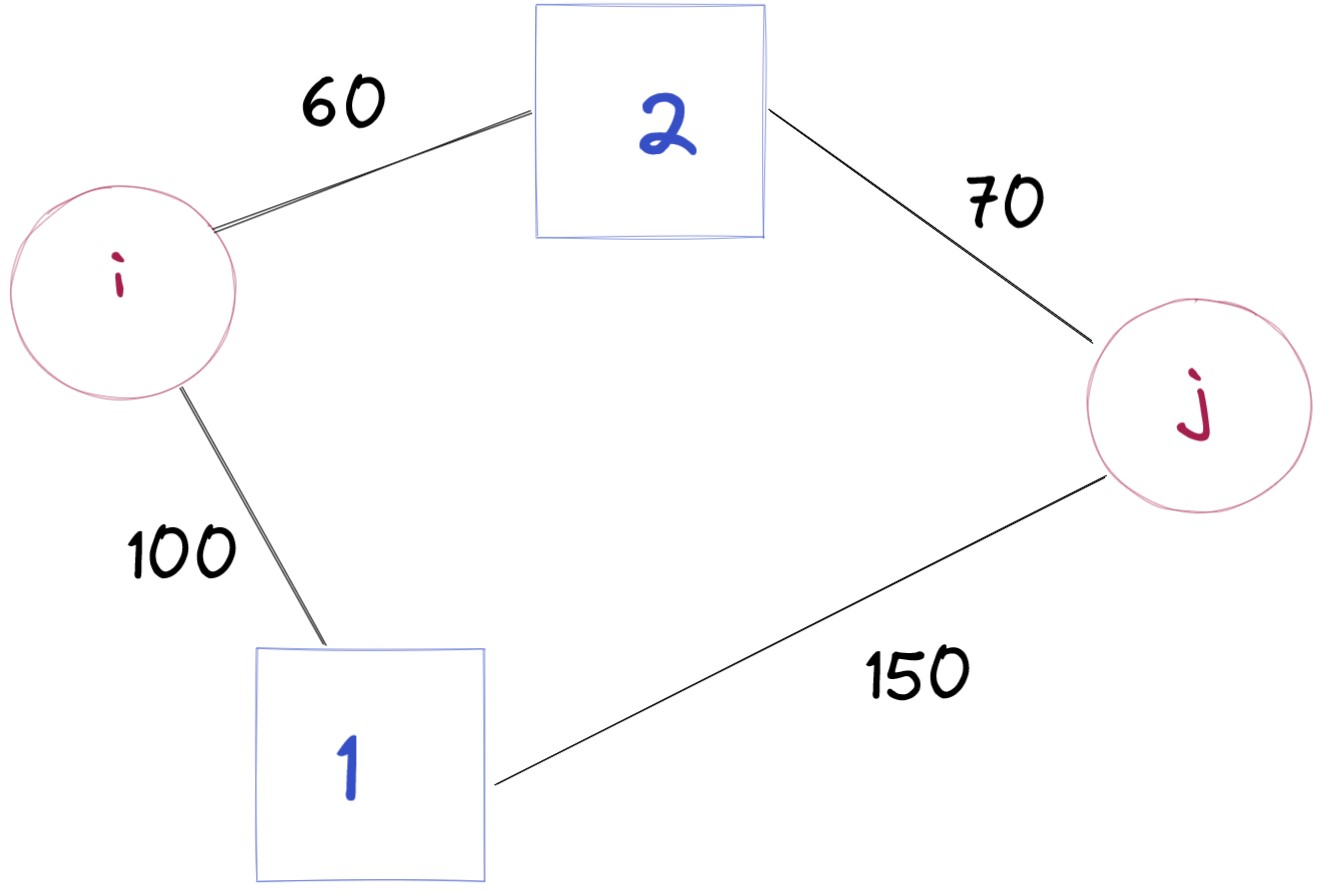
\includegraphics[scale=0.25]{datos_1_opp}
    \end{figure}
\end{frame}

\begin{frame}{Cost of Opportunity}
    \framesubtitle{Explanation}
    Following the minimization of distances approach, the assignments would be:
    \begin{figure}
        \centering
        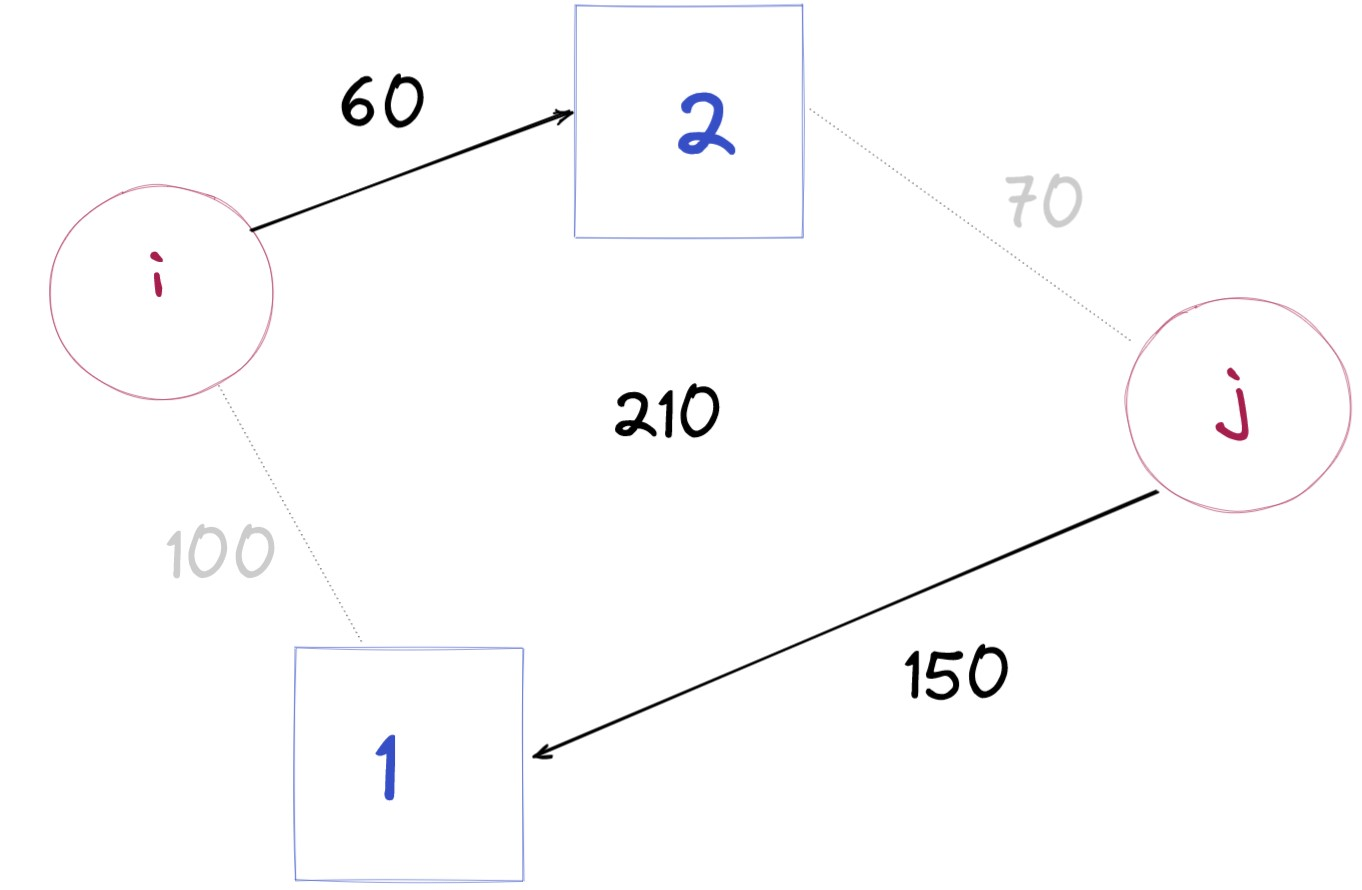
\includegraphics[scale=0.25]{Screenshot_1}
    \end{figure}
\end{frame}
\begin{frame}{Cost of Opportunity}
    \framesubtitle{Explanation}
    However, we may calculate the cost of opportunity as the difference between the optimal assignment and all the other possible assignments, selecting the largest opportunity lost:
    \begin{figure}
        \centering
        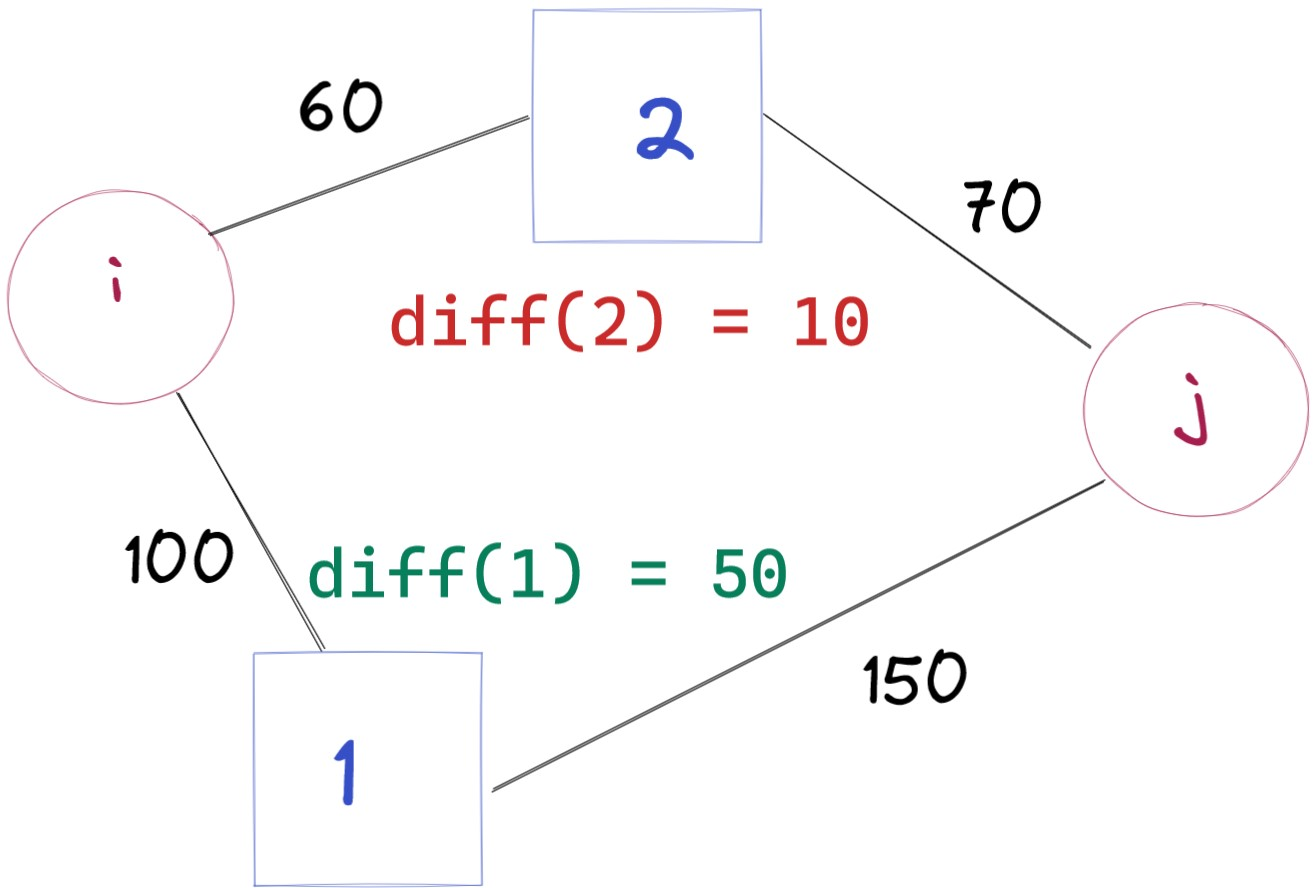
\includegraphics[scale=0.25]{Screenshot_2}
    \end{figure}
\end{frame}

\begin{frame}{Cost of Opportunity}
    \framesubtitle{Explanation}
    However, we may calculate the cost of opportunity as the difference between the optimal assignment and all the other possible assignments, selecting the largest opportunity lost:
    \begin{figure}
        \centering
        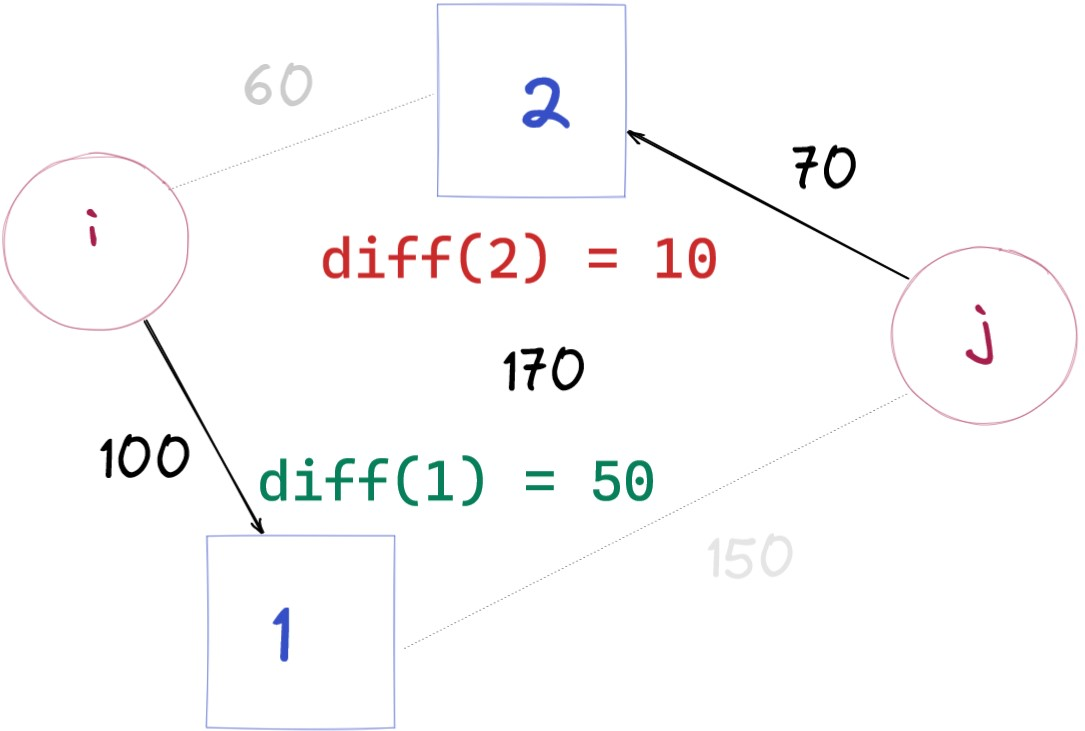
\includegraphics[scale=0.25]{Screenshot_3}
    \end{figure}
\end{frame}


\begin{frame}{Cost of opportunity}
    \scalebox{0.41}{
    \begin{minipage}{1.8\linewidth}
        \begin{algorithmic}[1]
            \REQUIRE $D, P, Y, S, B, n $, Instance
            \ENSURE $X$ := binary decision variable
            \STATE $C \gets D$
            \STATE $N \gets [i, \forall i \in Y_i == 0]$
            \FORALL{$j \in B$}
                \STATE $i' \gets$ argmin$(D[:,i]), i \notin N$
                \STATE $C[i,j] \gets D[i,j] - D[i',j], \forall i \in 1...S $
            \ENDFOR
            \STATE DONE $ \gets FALSE$
            \WHILE {NOT DONE}
                \STATE $CONS \gets [  ] $
                \STATE IDXS $\gets$ argmax$(C, n)$
                \FORALL{IDX $\in$ IDXS}
                \IF{IDX $\notin N$}
                    \STATE ROW $\gets$ find$(C[:, IDX] = 0)$
                    \STATE $X' \gets X$
                    \STATE $X'[ROW, IDX] \gets 1$
                    \STATE $CONS \gets \left( ROW, IDX, constraints(Instance, X') \right)$
                \ENDIF
                \STATE $i* \gets$ argmin(CONS)
                \IF{CONS[i*] = 0}
                    \STATE $ROW, COL \gets CONS[i*]$
                    \STATE $X[ROW, COL] \gets 1$
                \ELSE
                    \STATE $Candidates \gets argmin(C[:,i*], P/4)$
                    \STATE $CONS\_INNER \gets [ ]$
                    \FOR{Candidate $\in$ Candidates}
                        \STATE $X* \gets X$
                        \STATE $X*[Candidate, i*] \gets 1$
                        \STATE $CONS\_INNER \gets \left( ROW, IDX, constraints(Instance, X*) \right)$
                    \ENDFOR
                    \STATE $j* \gets argmin(CONS\_INNER)$
                    \STATE $ROW \gets CONS\_INNER[j*]$
                    \STATE $COL \gets CONS[i*]$
                    \STATE $X[ROW,COL] \gets 1$
                \ENDIF
                \STATE $D[:,COL] \gets \emptyset$
                \ENDFOR
                \STATE DONE $\gets$ Are All BUs Assigned?
            \ENDWHILE
            \RETURN $X$
        \end{algorithmic}
    \end{minipage}%
    }
\end{frame}

\begin{frame}{Upper Constraints Check}
    \scalebox{1}{
    \begin{minipage}{1.8\linewidth}
        \begin{algorithmic}[1]
            \REQUIRE Instance, X
            \ENSURE $cons$ := Number of violated constraints
            \FOR{Constraint in Constraints}
                \STATE $Violated \gets$ Check(Instance.parameters, Solution)
                \IF{Violated}
                    \STATE $cons += 1$
                \ENDIF
            \ENDFOR
            \RETURN $cons$
        \end{algorithmic}
    \end{minipage}%
    }
\end{frame}



\begin{frame}{Local search}
    \scriptsize Taking into consideration that the solution provided by the Constructive Heuristic needs to be "repaired", the local search moves first try to minimize constraints violated.
        \begin{block}{BU\_SimpleReassign($\psi, \tau$)}
        \centering
         \footnotesize Move a BU $j$ from center $\psi$ to the center $\tau$, where $\psi \ne \tau$
    \end{block}
    \begin{block}{BU\_Interchange($\psi, \tau$)}
        \centering \footnotesize
        Interchange the assignments of BUs $\psi$ and $\tau$
    \end{block}
    \begin{block}{Center\_SimpleReassign($\psi, \eta$)}
        \centering \footnotesize
        Change $Y_\psi$ from 1 to 0 and $Y_\eta$ from 0 to 1, allocate all the orphaned BUs from center $\psi$ to $\eta$ 
    \end{block}
    \begin{block}{Center\_SmartReassign($\psi, \eta$)}
        \centering \footnotesize
        Change $Y_\psi$ from 1 to 0 and $Y_\eta$ from 0 to 1, allocate all the orphaned BUs from center $\psi$ using the same allocation process of the Cost of Opportunity strategy.
    \end{block}
    
\end{frame}

\section{Empirical work}

\begin{frame}{Experiments layout}
    \framesubtitle{Computational results}
    The heuristics were coded in Julia 1.8
    The source code can be found in the following repository: \url{https://github.com/eduardosalaz/tesis}.\\
    The platform is Intel Core i5-9300 2.5 GHz, 8 GB RAM under Windows 10.
    For the experiments, instances were generated with BUs and Centers' coordinates located randomly between 5 and 4500 along with the center types, risk and activity measures.
\end{frame}

\begin{frame}{Constructive algorithms comparison}
    \framesubtitle{Computational results}

    \begin{block}{Data set}
        \begin{description}
            \item[Size 1] 25 instances with 310 BUs, 60 centers and 20 to be located.
            \item[Size 2] 10 instances with 800 BUs, 150 centers and 50 to be located.
        \end{description}
    \end{block}
\end{frame}

\begin{frame}{Constructive algorithms comparison}
    \framesubtitle{Computational results}
    \begin{table}
        \centering
        \scalebox{0.67}{
        \begin{tabular}{c|c|c|c|c|c|c|c|c|c|c|c|}
            \hline
            \multicolumn{3}{c}{Inst.} &
            \multicolumn{1}{c}{Loc.} &
            \multicolumn{2}{c}{Avg. constraints} &
            \multicolumn{2}{c}{\% Factible sols.} &
            \multicolumn{2}{c}{Avg. time alloc. (s)} &
            \multicolumn{1}{c}{Avg. time loc. (s)} \\ \hline
            $B$ & $S$ & $P$ & & N & C & N & C & N & C & \\ \hline
            \multirow{3}{*}{310} & \multirow{3}{*}{60} & \multirow{3}{*}{20} & Rlx & 5.92 & 0.08 & 0 & 96 & 0.004 & 2.05 & 1.2\\ & & & Pdp & 42.2 & 8.44 & 0 & 0 & 0.005 & 1.114 & 0.0006 \\ & & & Rnd & 21.76 & 4.92 & 0 & 0 & 0.004 & 0.954 & 0 \\ \hline
            \multirow{3}{*}{800} & \multirow{3}{*}{150} & \multirow{3}{*}{50} & Rlx & 12.4 & 0 & 0 & 100 & 0.014 & 47.7 & 16.6\\ & & & Pdp & 102.4 & 19.4 & 0 & 0 & 0.016 & 69.54 & 0.0009 \\ & & & Rnd & 43.5 & 8.9 & 0 & 0 & 0.013 & 56.84 & 0 \\ \hline
        \end{tabular}}
        \caption{Summary of the experiment results}
        \label{tab:constructive_exp}
    \end{table}
    
    Based on these results, it was decided to use the Integer Relaxation as the Location Phase and the Opportunity Cost as the Allocation Phase for the Constructive Phase of the GRASP Procedure.
\end{frame}
\begin{frame}{Constructive algorithms comparison}
    \framesubtitle{Comparison with the Solver}
    \begin{table}
        \centering
        \scalebox{1}{
        \begin{tabular}{c|c|}
            \hline
            Dataset & Avg. Gap\% to Optim \\ \hline
            1 & 51.7\\ \hline
            2 & 51.2\\ \hline
        \end{tabular}}
        \caption{Summary of the experiment results}
        \label{tab:constructive_optim_comp}
    \end{table}
    Part of the methodology of the experiments involved programming the model in order to feed it to an exact solver, in this case CPLEX to provide a baseline of the optimal value and how much time it takes to solve with a cutoff time of 300 seconds.
\end{frame}
\begin{frame}{Local Search algorithms comparison}
    \framesubtitle{Computational results with violated constraints}
    \begin{table}
        \centering
        \scalebox{0.7}{
        \begin{tabular}{c|c|c|}
            \hline
            Dataset & Move & Avg. constraints improv. \% \\ \hline
            \multirow{4}{*}{1} & BU\_Simple & 39.31 \\ & BU\_Interchange & 0\\ & Center\_Simple & 6.22\\ & Center\_Smart & 8.03\\ \hline
            \multirow{4}{*}{2} & BU\_Simple & 29.63\\ & BU\_Interchange & 0\\ & Center\_Simple & 2.67 \\ & Center\_Smart & 0\\ \hline
        \end{tabular}}
        \caption{Summary of the experiment results}
        \label{tab:ls_cons_exp}
    \end{table}
    With the application of the local search focused on minimizing the number of constraints violated in unfactible solutions, we find that there is an improvement on the value mainly coming from the BU\_Simple move, whereas BU\_Interchange proves inefective.
\end{frame}

\begin{frame}{Local Search algorithms comparison}
    \framesubtitle{Computational results}
    \begin{table}
        \centering
        \scalebox{0.7}{
        \begin{tabular}{c|c|c|c|}
            \hline
            Dataset & Move & Avg. Time & Avg. rel. improv. \% \\ \hline
            \multirow{4}{*}{1} & BU\_Simple & 4.4 & 48.35 \\ & BU\_Interchange & 2.09 & 2.94 \\ & Center\_Simple & 66.4 & 0.02 \\ & Center\_Smart & 1.68 & 0 \\ \hline
            \multirow{4}{*}{2} & BU\_Simple & 16.5 & 48.32 \\ & BU\_Interchange & 1.67 & 1.67 \\ & Center\_Simple & 15.68 & 0 \\ & Center\_Smart & 31.12 & 0 \\ \hline
        \end{tabular}}
        \caption{Summary of the experiment results}
        \label{tab:ls_improv_exp}
    \end{table}
    Each Move had a fixed number of iterations, for the first dataset, $max\_iters = 1000:1500$ but we suspect there is a bug somewhere, as for the same number of iterations, the second dataset would OOM the procedure, so $max\_iters$ had to be lowered to $200:250$.
    Based on these results, it was decided to use BU\_Simple and BU\_Interchange moves in the GRASP procedure with around 200 iterations for each move.
\end{frame}

\begin{frame}{Constructive and Local Search comparison}
    \framesubtitle{Comparison with the Solver}
    \begin{table}
        \centering
        \scalebox{1}{
        \begin{tabular}{c|c|}
            \hline
            Dataset & Avg. Gap\% to Optim\\ \hline
            1 & 5.86 \\ \hline
            2 & 5.25 \\ \hline
        \end{tabular}}
        \caption{Summary of the experiment results}
        \label{tab:constructive_ls_optim_comp}
    \end{table}
    Even though there is a considerable improvement in the objective function, not all moves are useful for improving the objective function value.
\end{frame}

\begin{frame}{GRASP Pseudocode}
        \begin{algorithmic}[1]
        
        \REQUIRE $P, \alpha, \gamma, i_{max}$, Instance
        \ENSURE $X,Y$ = binary decision variables
        
        \STATE $A^* \gets \emptyset$
        \STATE $f^* \gets \infty$
        \WHILE {$i_{max} > 0$}
            \STATE $X, Y \gets$ Construct($\alpha, P$, Instance)
            \STATE $X, Y \gets$ LocalSearch($X, Y,$ Instance)
            \STATE $A \gets (X, Y)$
            \IF {$f(A) < f^*$}
                \STATE $f^* \gets f(A)$
                \STATE $A^* \gets A$ 
            \ENDIF
            \STATE $i_{max} \gets i_{max} - 1$
        \ENDWHILE
        \RETURN $A^*$
        \end{algorithmic}
\end{frame}

\begin{frame}{Construct Pseudocode}
\scalebox{0.33}{
\begin{minipage}{1.5\linewidth}
\begin{algorithmic}[1]
        \REQUIRE $P, \alpha, \gamma,$, Instance
        \ENSURE $X,Y$ = binary decision variables
        \STATE $Y \gets IntegerRelaxation(Instance)$
        \STATE $Y' \gets$ Perturbate Y (turn off $\gamma$ centers previously on and turn on $\gamma$ centers previously off)
        \STATE $C \gets D$
            \STATE $N \gets [i, \forall i \in Y_i == 0]$
            \FORALL{$j \in B$}
                \STATE $i' \gets$ argmin$(D[:,i]), i \notin N$
                \STATE $C[i,j] \gets D[i,j] - D[i',j], \forall i \in 1...S $
            \ENDFOR
            \STATE DONE $ \gets FALSE$
            \WHILE {NOT DONE}
                \STATE $CONS \gets [  ] $
                \STATE IDXS $\gets$ argmax$(C, n)$
                \FORALL{IDX $\in$ IDXS}
                \IF{IDX $\notin N$}
                    \STATE ROW $\gets$ find$(C[:, IDX] = 0)$
                    \STATE $X' \gets X$
                    \STATE $X'[ROW, IDX] \gets 1$
                    \STATE $CONS \gets \left( ROW, IDX, constraints(Instance, X') \right)$
                \ENDIF
                \STATE $i* \gets$ argmin(CONS)
                \IF{CONS[i*] = 0}
                    \STATE $ROW, COL \gets CONS[i*]$
                    \STATE $BestVal \gets C[ROW, COL]$
                    \STATE $Cutoff \gets (BestVal + (BestVal * \alpha))$
                    \STATE $RCL \gets [IDX if C[IDX] <= Cutoff]$
                    \STATE $ROW, COL \gets Rand(RCL)$ 
                    \STATE $X[ROW,COL] \gets 1$
                \ELSE
                    \STATE $BestVal \gets C[ROW, COL]$
                    \STATE $Cutoff \gets (BestVal + (BestVal * \alpha))$
                    \STATE $RCL \gets [IDX if C[IDX] <= Cutoff]$
                    \STATE $i* \gets Rand(RCL)$
                    \STATE $Candidates \gets argmin(C[:,i*], P/4)$
                    \STATE $CONS\_INNER \gets [ ]$
                    \FOR{Candidate $\in$ Candidates}
                        \STATE $X* \gets X$
                        \STATE $X*[Candidate, i*] \gets 1$
                        \STATE $CONS\_INNER \gets \left( ROW, IDX, constraints(Instance, X*) \right)$
                    \ENDFOR
                    \STATE $j* \gets argmin(CONS\_INNER)$
                    \STATE $ROW \gets CONS\_INNER[j*]$
                    \STATE $COL \gets CONS[i*]$
                    \STATE $X[ROW,COL] \gets 1$
                \ENDIF
                \STATE $D[:,COL] \gets \emptyset$
                \ENDFOR
                \STATE DONE $\gets$ Are All BUs Assigned?
            \ENDWHILE
            \RETURN X, Y
        \end{algorithmic}
        \end{minipage}%
        }
\end{frame}


\begin{frame}{Calibrating GRASP iterations}
    \framesubtitle{Computational results}
    
    In order to gain insight about when the solutions yielded by the GRASP algorithm stop improving, we run an experiment with $i_{max} = 50$ and $\alpha = 0.2, 0.3, 0.4$ for the objective function average of 5 instances of the first dataset.
    
    \begin{figure}
        \centering
        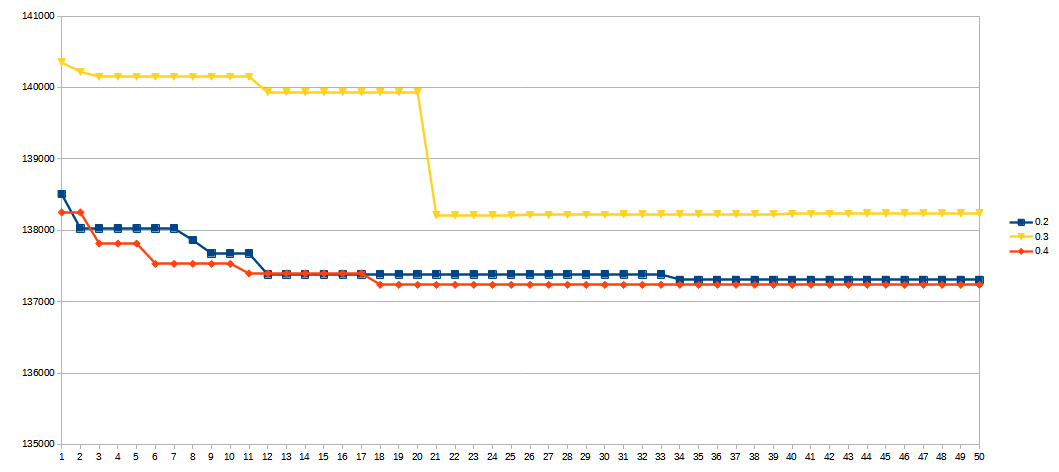
\includegraphics[scale=0.3]{resultados_alfa}
    \end{figure}
\end{frame}

\begin{frame}{GRASP runtime}
    \framesubtitle{Computational results}
    As we tested the GRASP procedure speed, we found the following results:

    \begin{table}
        \centering
        \scalebox{0.7}{
        \begin{tabular}{c|c|c|c|c|c|}
            \hline
            Dataset & Loc. time & Alloc. time. & Move time. & Avg. rel. improv. \% & Avg. Gap\% to optim\\ \hline
            1 & 2.1  & 23 & 8.4 & 49.21 & 2.9 \\ \hline
            2 & 17.5 & 40.6 & 20.6 & 47.34 & 5.2\\ \hline
        \end{tabular}}
        \caption{Summary of the experiment results}
        \label{tab:grasp_optim_comp}
    \end{table}
   
\end{frame}

\begin{frame}{Comparing GRASP with the Exact Solver}
    \framesubtitle{Computational results}
    With an $\alpha = 0.3$ and 30 iterations, we decided to try and solve larger instances to test the capabilities of the metaheuristic. So, the last test dataset consisted of a single instance with 1300 BUs, 190 centers and $P$ = 65. The solver did not finish optimally at the cutoff of 300 seconds, whereas the GRASP ran out of memory at the third iteration. Still, the GRASP took 86 seconds to provide a solution within 3.7\% of the solver's solution.
\end{frame}



\section{Wrap-up}

\begin{frame}{Wrap-up}
    \small Conclusions
    \scriptsize
    \begin{itemize}
        \item Using an integer relaxation of the problem and the cost of opportunity assignment we get factible solutions from the constructive heuristic, with the simple BU reassignment move proving the most effective for the Local Search.
        \item On fine-tuning stage of GRASP, it was observed that a value of $i_{max} = 30, \alpha = 0.3$ was good enough
        \item GRASP provides good solutions, however the time and memory spent in the local search phase made it unfeasible to test on larger instances.
    \end{itemize}
    \small Future work
    \scriptsize
    \begin{itemize}
        \item Explore the usage of P-Dispersion as the Location Phase instead of Relaxation.
        \item Optimize code, profile performance, detect bottlenecks and memory leaks
        \item Improve the algorithm data structures to reduce running times
        \item Explore other location phase heuristics
        \item Explore other strategies (TS, ILS, IGLS, VNS, SS)
    \end{itemize}
\end{frame}

\begin{frame}{Acknowledgments}
    \begin{itemize}
        \item Thank you very much for your attention!
        \item Feedback is welcome :)
        \item Email: eduardosalaz@outlook.com
        \item GitHub: \url{https://github.com/eduardosalaz}
    \end{itemize}
    
    \begin{figure}
        \centering
        
\includegraphics[scale=0.2]{uanl-logo}
        
\includegraphics[scale=0.2]{fime-logo}
    \end{figure}
\end{frame}

\begin{frame}{References}

\printbibliography
\end{frame}
\end{document}